
\documentclass[extendedabs]{AAVL}

\runninghead{Claus, Fitzgibbon}{Plumbline Constraint for the RF Model}

\begin{document}

\title{Numerical simulations for selected 1D and 2D Mass-spring
models and Applications}

\addauthor{Sachin Chandrasekara}{SC/2018/10559}{1}


\addinstitution{
Department of Mathematics,\\
Faculty of Science,\\
University of Ruhuna}

\maketitle
\section{Problem statement}
\label{aa}

\noindent
Considering the our project title, the first assignment was given by our supervisor to do a free spring-mass model to two degrees. We were given below figure \ref{fig:b} and we had to create a MATLAB model considering that. 
\begin{figure}[hbt!]
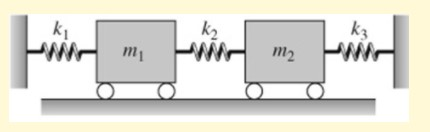
\includegraphics[width=\linewidth]{images/b.jpg}
\caption{Two DOF spring mass }
\vspace{-2mm}
\label{fig:b}
\end{figure}

\section{Approach}
In this section, I have described some of the theories and assumptions I have already used. 
\subsection{Degree of freedom}
The degree of freedom for a dynamic system is the number of directions in which a particle can move freely or the total number of coordinates required to describe completely the position and configuration of the system. It is denoted by $N$. Degree of freedom of a system is given by, 
\begin{equation}
    N = 3*A-R
\end{equation}
$A$ = number of particles in the system \\
$R$ = number of independent relations between the particles

In given figure \ref{fig:b} Degree of freedom (DOF) = 3*2-4 =2, Therefore we can say in the figure \ref{fig:b} two body degree of freedom.
\subsection{The Euler-Lagrange equations}
\label{ab}
Here is the procedure. Consider the following seemingly silly combination of the kinetic and potential energies ($T$ and $V$ , respectively), It is denoted by $L$,
\begin{equation}
\label{aaa}
    L = T-V
\end{equation}

In the section \ref{aa}, figure \ref{fig:b} is a two degree of freedom system, governed by two differential equations. The governing equations can also be achieved by following Lagrange's Equation directly. The expression for kinetic energy is,
\begin{equation}
    T = \frac{1}{2}m_1\dot{x_1}^2 + \frac{1}{2}m_2\dot{x_2}^2
\end{equation}
And also, the expression for potential energy is,
\begin{equation}
    V = \frac{1}{2}k_1x^2+\frac{1}{2}k_2(x_2-x_1)^2+\frac{1}{2}k_3x_3^2
\end{equation}
Applying Lagrange’s equation to equation \eqref{aaa},
\begin{equation}
    \frac{d}{dt}(\frac{\partial L}{\partial \dot{x1}})-\frac{\partial L}{\partial x1} = 0 
\end{equation}
\begin{equation}
     \frac{d}{dt}(\frac{\partial L}{\partial \dot{x1}})-\frac{\partial L}{\partial x1} = 0
\end{equation}

\subsection{Governing equations}
Governing differential equations are based on balance laws for mass and momentum, and completed by constitutive relations for the fluid and solid phases as well as their mutual interactions. In the section \ref{ab} its results we can obtain the governing equations as,

\begin{equation}
\label{aab}
    m_1\dot{x_1}+(k_1+k_2)x_1-k_2x_2=0
\end{equation}
\begin{equation}
\label{aac}
    m_2\dot{x_2}-k_2x_1+(k_2+k_3)x_2 = 0
\end{equation}
Clearly, for multi degree of freedom systems, this approach has advantages over the force balancing approach
using Newton’s law.
\subsection{Matrix form of equations of motion}
The matrix form of the system of governing equations of motion is as follows and the component matrices are commonly named as listed below.
\begin{equation}
\label{aad}
    [M]{\dot{X}}+[K]{X} = 0
\end{equation}
$M$ =Inertia matrix \\
$K$ =Stiffness matrix\\
$X$ =Displacement vector\\
$\dot{X}$=Velocity vector

These matrices describe a set of "n" linear second order ordinary differential equations, where "n" is the number of degrees of freedom in the system. Where the solutions involved with equations \eqref{aab} and \eqref{aac},

\begin{gather}
    \begin{bmatrix}
m_1 & 0\\0& m_2 
\end{bmatrix}{\dot{X}} +
\begin{bmatrix}
(k_1+k_2)&-k_2\\-k_2&(k_2+k_3)
\end{bmatrix}{X} = 0
\end{gather}

The solution $x(t)$ in the form of harmonic oscillations,
\begin{equation}
    x(t) = \sum x_ie^{jw_it}
\end{equation}

If for that frequency we build all our displacements into a vector, ${x}$, then its second derivative will be,
\begin{equation}
    {\Ddot{x}} = w^2{x}
\end{equation}
So we can substitute this into equation \eqref{aad}
\begin{equation}
    ([K]^{-1}[K] -\omega^2[I]){x} = 0
\end{equation}

For each of these frequencies we can find the corresponding eigenvector {x} which will represent a mode of the system. where [I] is the unit matrix.

\subsection{The Eigenvalue}
In this case, the matrix $M$ is just a diagonal set of numbers representing each of the masses.
\begin{gather}
    det\begin{vmatrix}
    [K]-\omega^2[M]
    \end{vmatrix}=0
\end{gather}
The roots of the polynomial expression of the determinant are the  eigenvalues of the matrix $M^{-1}K$ and there will be two such solutions in our 2-DOF system, so there will be two natural frequencies. The convention is to then sort the eigenvalues into ascending order so that you talk about the first natural frequency (the lowest) and the second, etc.

\section{Further work}
Considering above mentioned mathematical assumption, the first MATLAB code was made up of files as Code1 and SolCode1. Furthermore, you can go to my GitHub account \url{https://github.com/sachinkavindaa/IM-Project-Level_2} and all the update files are there.





 
  


\end{document}
